% !TEX program = xelatex

\documentclass[a4paper,scheme=chinese,linespread=1.5]{ctexbook} % 行距固定值20磅
\usepackage[a4paper, top=2.54cm, bottom=2.54cm, left=3.18cm, right=3.18cm]{geometry} %页边距 左右3.18cm 上下2.54cm
\setlength{\parskip}{0pt}  % 手动控制段落间距 

\usepackage{ctex}
\usepackage{arydshln} 

\usepackage{amsmath}
\usepackage{amssymb}

%\usepackage{newtxtext, newtxmath}

%伪代码
\usepackage{algorithm}
\usepackage{algorithmic}
%\usepackage{algpseudocode}

\usepackage{xeCJK}
\usepackage{xeCJKfntef}

\usepackage{fancyhdr}

\usepackage{tikz}
\usepackage{graphicx}

\usepackage{enumitem}
\usepackage{ragged2e}

%五线谱包,可以用西贝柳斯+pdf代替
%\usepackage{musixtex}

\usepackage{float}
\usepackage{xcolor}

% 设置页脚
\pagestyle{fancy}
\fancyhf{}  % 清空页眉和页脚
\renewcommand{\headrulewidth}{0pt} % 去除页眉横线
\renewcommand{\footrulewidth}{0pt} % 如果页脚横线也不需要,可以设置为 0pt

%导入加载图片库
\usepackage{graphicx}
\usepackage{multicol}

\newcommand{\fixeduline}[2][8cm]{\uline{\makebox[#1]{#2}}}

\newcommand{\degree}{硕}%博 / 硕
\newcommand{\chimaintitle}{中文标题}
\newcommand{\chisubtitle}{——中文副标题} % 中文副标题 如果不用就去了 -> \newcommand{\chisubtitle}{}
\newcommand{\engtitle}{English Title}

%导入时间
\usepackage{datetime2}

\usepackage{xparse}

%表格
\usepackage{longtable}
\usepackage{multirow}
\usepackage{booktabs}

%导入中文文献引用标准 GB/T 7714
\usepackage{gbt7714}
\bibliographystyle{gbt7714-numerical}

\newcommand*\circled[1]{\tikz[baseline=(char.base)]{
		\node[shape=circle,draw,inner sep=1.2pt] (char) {#1};}
} 

%阿拉伯对应中文数字的转换
\newcommand{\chinesenumber}[1]{%
	\ifcase#1 零 \or 一\or 二\or 三\or 四\or 五\or 六\or 七\or 八\or 九\or 十\fi
}

%\usepackage{ctex}
%\ctexset{chapter/name={第,章}, chapter/font=\Large\bfseries}

\NewDocumentCommand{\addchapter}{s m}{%
	\IfBooleanTF{#1}
	{
		%\chapter*
		{
			\centering
			\heiti
			\zihao{-2}
			\hspace*{-0.75em}
			\selectfont #2
			\vspace*{1em}

			
		}
	} % * 不放进目录
	{
		%\chapter*
		\stepcounter{chapter}
		{
			\zihao{-2}
			\vspace*{-0.75em}
			\begin{center}
				第\chinesenumber{\value{chapter}}章、#2
			\end{center}
			\vspace*{-1em}
		}
		%\vspace*{-\baselineskip}
		
		\addcontentsline{toc}{chapter}{#2}
		
	} % 放进目录
}

%页面设置
\usepackage{titlesec}
\usepackage{tocloft}
%\usepackage{fontspec}
%\usepackage[subfigure]{tocloft}

% 自定义 目录
\setcounter{tocdepth}{4}
\renewcommand{\contentsname}{\vspace*{-0.75em} \hfill \zihao{-2}\color{black}目\hspace*{0.75em}录 \hfill}  % 修改目录的标题 居中 小二 黑体

\renewcommand{\cftchapleader}{\cftdotfill{\cftdotsep}} % 目录加省略号

\setlength{\cftsecindent}{3.5em}  % 设置 section 的缩进为 3.5em
\setlength{\cftsubsecindent}{5.5em}  % 设置 subsection 的缩进
\setlength{\cftsubsubsecindent}{7.5em}  % 设置 subsection 的缩进

\setlength{\cftsecnumwidth}{4em}  % 设置章节编号宽度
\setlength{\cftsubsecnumwidth}{4em}  % 设置子章节编号宽度
\setlength{\cftsubsubsecnumwidth}{4em}  % 设置子章节编号宽

% 超链接
\usepackage{xcolor}
\usepackage{hyperref}
\hypersetup{
	pdfborder={0 0 0},        % 边框为无(无边框)
	colorlinks=false,          % 启用彩色链接
	linkcolor=white,           % 章节、表格、图形的链接颜色
	citecolor=white,           % 引用的链接颜色
	urlcolor=white,            % URL 的链接颜色
	pdfauthor={},             % 作者
	pdftitle={},              % 标题
	pdfsubject={},            % 主题
	pdfkeywords={},           % 关键词
	pdfcreator={},            % 创建者
	pdfproducer={},           % 生产者
	%linkbordercolor=black,      % 设置链接的边框颜色
	%urlbordercolor=black,           % 设置URL的边框颜色
	%citebordercolor=black,            % 设置引用的边框颜色
	%pdfborderstyle={/S/D/D[3 2]/W 1} % 虚线
}

% 脚注
\usepackage{pifont}  % 引入宏包pifont
\usepackage{footnote}
\usepackage[perpage]{footmisc}

% 需结合计数器调整:
\renewcommand{\thefootnote}{%
	\ifnum\value{footnote}<11 
	\raisebox{0.35ex}{\scalebox{0.75}{\ding{\numexpr 171+\value{footnote}}}}% 缩放符号 ①~⑩
	\else 
	\textcircled{\scriptsize\arabic{footnote}}% 超过11时改用其他方式
	\fi}


% 自定义 section 标题:第x节
\renewcommand{\thesection}{第\chinesenumber{\value{section}}节}
\titleformat{\section}%[block]
{	
	\centering
	\raggedright
	\zihao{-3}
}
{}{0em}{}
\newcommand{\DIYsection}[1]{
	\stepcounter{section}
	%
	\section*{
		\zihao{-3}
		\begin{center}
			\thesection、
			#1
		\end{center}
		\vspace*{-2.5em}
	}
	
	\addcontentsline{toc}{section}{\thesection \quad #1}
}

% 自定义 subsection 标题:第x小节 [可自行修改]
\renewcommand{\thesubsection}{第\chinesenumber{\value{subsection}}小节}
\titleformat{\subsection}%[block]
{	
	\raggedright
	\songti
	\zihao{-3}
	\color{black}
}
{}{0em}{}
\newcommand{\DIYsubsection}[1]{
	\stepcounter{subsection}
	\subsection*{\thesubsection、#1}
	\addcontentsline{toc}{subsection}{\quad #1}
}


%图表注释
\usepackage{caption}
\captionsetup{labelfont={rm, bf,color=black},textfont={rm,bf}}

%图表脚注
\usepackage{tablefootnote}

%字体设置
\newCJKfontfamily\huawenzhongsong{STZHONGS}[BoldFont=STZHONGS, Path=./fonts/, Extension=.TTF] %华文中宋
\setmainfont{Times New Roman} % 设置西文字体 
\setCJKmainfont[
BoldFont = SimHei
]{SimSun}       % 设置中文字体为宋体 




\begin{document}

	% TODO 封面信息
	\begin{titlepage}
		\begin{center}
			\noindent
			
\includegraphics[width=0.6\textwidth]{figures/ccom/ccom_logo.eps}\vspace{2cm}
		\end{center}
		
		
		\begin{center}
			{\fontsize{36pt}{36pt}\fontfamily{微软雅黑}\selectfont \degree~\:士~\:学~\:位~\:论~\:文}\vspace{2cm}
			
			{ \heiti \fontsize{32pt}{32pt}\selectfont\bfseries \chimaintitle \protect\\
				\vspace*{0.25em}
				\fontsize{28pt}{28pt}\selectfont\bfseries \chisubtitle \par}%\vfill
			
			\vspace*{10em}
			{\LARGE\huawenzhongsong
				作者姓名:\fixeduline{匿名}\\
				学  号:\fixeduline{2XXXXX}\\
				所在系部:\fixeduline{音乐人工智能与音乐信息科技}\\
				研究方向:\fixeduline{音乐人工智能与音乐信息科技}\\
				导师姓名:\fixeduline{YF~教授、XXX~教授}\\
				提交时间:\fixeduline{20XX年04月}\\
			}
		\end{center}
		
	\end{titlepage}
	
	% TODO 论文原创性声明和使用授权书
	{\large
		
		\setlength{\columnsep}{0pt}
		
		{
			\centering 
			\fontsize{16pt}{16pt}
			\heiti{中央音乐学院\degree 士学位论文原创性声明}\par
		}
		
		\vspace{0.3cm}
		
		本人郑重声明:此处所提交的\degree 士学位论文\kaishu \uline{\,《\chimaintitle\chisubtitle》} \songti ,是本人在导师指导下,在中央音乐学院攻读\degree 士学位期间独立进行研究工作所取得的成果。据本人所知,论文中除已注明部分外不包含他人已发表或撰写过的研究成果。对本文的研究工作做出重要贡献的个人和集体,均已在文中以明确方式注明并表示了谢意。本声明的法律结果将完全由本人承担。
		
		\begin{multicols}{2}
			\vfill\null
			\columnbreak
			\heiti{作者签名:}~~~~%\raisebox{-0.2\height}{\includegraphics[width=1.25cm, height=0.65cm ]{figures/signatures/sy.pdf}} %括号里是作者电子签
			\par
			\vspace{0.3cm}
		\end{multicols}
		
		\hfill \heiti{\the\year~年~\the\month~月~\the\day~日}
		\vfill
		
		{
			\centering 
			\fontsize{16pt}{16pt}
			\heiti{中央音乐学院\degree 士学位论文使用授权书}\par
		}
		
		\vspace{0.3cm}
		
		\songti
		
		\kaishu \uline{\,《 {\chimaintitle\chisubtitle}》} \songti 系本人在中央音乐学院攻读\degree 士学位期间在导师指导下完成的\degree 士学位论文。本人完全了解中央音乐学院关于保存、使用学位论文的规定,同意学校保留并向有关部门送交论文的复印件和电子版本,允许论文被查阅和借阅。
		
		\begin{multicols}{2}
			\vfill\null
			%\columnbreak
			\heiti{作者签名:}~~~~%\raisebox{-0.25\height}{\includegraphics[width=1.25cm, height=0.65cm ]{figures/signatures/sy.pdf}} %括号里是作者电子签
			
			\vspace*{0.3cm}
			\hfill \heiti{\the\year~年~\the\month~月~\the\day~日}
			\vfill
			
			\columnbreak
			
			\vfill\null
			
			\heiti{导师签名: }\raisebox{-0.35\height}{
\includegraphics[width=1.75cm, height=1cm ]{figures/signatures/yuyuan.pdf}} \quad %\raisebox{-0.25\height}{\includegraphics[width=1.75cm, height=1cm ]{figures/signatures/dls.pdf}} %二位导师签名
			
			\vspace*{0.3cm}
			\hfill \heiti{\the\year~年~\the\month~月~\the\day~日}
			
			\vfill
		\end{multicols}
		
		\vfill
		
		{
			\centering 
			\fontsize{16pt}{16pt}
			\heiti{中央音乐学院\degree 士学位论文使用授权书}\par
		}
		
		\vspace{0.3cm}
		
		本人授权中央音乐学院,可以将本论文提交中国学术期刊(光盘版)电子杂志社在《中国优秀博硕士学位论文数据库》中发表,可以采用影印、缩印或扫描等复制手段保存学位论文。
		
		\begin{multicols}{2}
			\vfill\null
			%\columnbreak
			\heiti{作者签名:}~~~~%\raisebox{-0.25\height}{\includegraphics[width=1.25cm, height=0.65cm ]{figures/signatures/sy.pdf}} %括号里是作者电子签
			
			\vspace*{0.3cm}
			\hfill \heiti{\the\year~年~\the\month~月~\the\day~日}
			\vfill
			
			\columnbreak
			
			\vfill\null
			
			\heiti{导师签名: }\raisebox{-0.35\height}{
\includegraphics[width=1.75cm, height=1cm ]{figures/signatures/yuyuan.pdf}} \quad %\raisebox{-0.25\height}{\includegraphics[width=1.75cm, height=1cm ]{figures/signatures/dls.pdf}} %二位导师签名
			
			\vspace*{0.3cm}
			\hfill \heiti{\the\year~年~\the\month~月~\the\day~日}
			
			\vfill
		\end{multicols}
		
		%\textbf{作者签名: }\raisebox{-0.25\height}{\includegraphics[width=1.25cm, height=0.65cm ]{figures/signatures/sy.pdf}} %括号里是作者电子签
		~~~~~~~~~~~~~~~
		%\textbf{导师签名: }\raisebox{-0.25\height}{
\includegraphics[width=0.125\columnwidth]{figures/signatures/yuyuan.pdf}} %\quad \raisebox{-0.25\height}{\includegraphics[width=1.75cm, height=1.15cm ]{figures/signatures/dls.pdf}} %二位导师签名
		%\par
		%\hspace*{5em} \textbf{\the\year~年~\the\month~月~\the\day~日}  \textbf{\the\year~年~\the\month~月~\the\day~日}
		%%%%%%%%%%%%%%%%%%%%%%%%%%%%%%%%%%%%
	}
	
	\newpage
	
	% 中文摘要
	\pagenumbering{Roman}
	\setcounter{page}{1}
	
	\addchapter*{论文摘要}
	\addcontentsline{toc}{chapter}{中文摘要}
	阿巴阿巴
	
	\textbf{关键词}: 
	chipichapa;tibodiibo
	
	\newpage
	
	% 英文摘要
	\addchapter*{\textbf{Abstract}}
	\addcontentsline{toc}{chapter}{英文摘要}
	blablabla
	
	\textbf{Key Words}: 
	chipichapa; tibodiibo
	
	\newpage
	
	%目录
	\tableofcontents
	
	\newpage
	
	%恢复页码
	\fancyhf{}
	\pagenumbering{arabic}
	\fancyfoot[C]{\thepage}
	\setcounter{page}{1}
	
	%绪论
	\addchapter{绪论}
	
	\DIYsection{研究背景与意义}
	
	脚注这样标\footnote{李伟、王鑫主编:《音频音乐与计算机的交融——音频音乐技术2》,上海:复旦大学出版社,2022年,第252-270页。}。
	
	% 这是图片
	\begin{figure}[H]
		\centering
		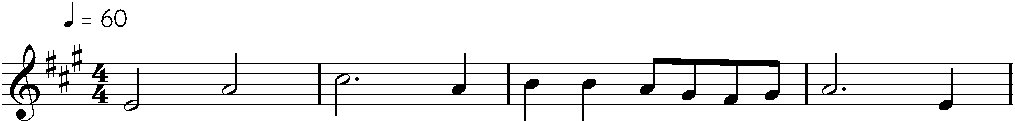
\includegraphics[width=1\textwidth]{figures/vio1_beeth2_1.pdf}  % 插入PDF文件
		\caption{图片标题}  % 图片标题
		\label{fig:1.1}  % 图片标签
	\end{figure}
	
	使用“\textbf{$\backslash \text{ref\{fig:1.x\}}$}"引用公式\ref{fig:1.1}。使用$\backslash \text{toprule}[\text{1.5pt}]$和$\backslash \text{bottomrule}[\text{1.5pt}]$来定义表格顶部和底部的线宽,使用$\backslash \text{midrule}[\text{0.75pt}]$定义中间线宽,以此基准制作三线格。可使用$\backslash \text{cmidrule}[{line\ width}]\{{number}_1-{number}_2\}$自定义线宽和占据的格数,如表\ref{tab:1.2}第三行所示。
	
	% 这是表格
	\begin{table}[h]
		\centering
		\caption{表格标题}
		\vspace*{-1em}
		\begin{tabular}{ccccccc}
			\toprule[1.5pt]
			Pitch (MIDI) & Onset & Duration  & String & Position & Finger & Type \\ \midrule[0.75pt]
			64           & 0     & 2         & 2 	  & 1 		 & 2 	  & 1 \\
			69           & 2     & 2         & 2 	  & 3		 & 3 	  & 1 \\
			73           & 0     & 3         & 2 	  & 3 		 & 5 	  & 1 \\
			69           & 3     & 1         & 2 	  & 3 		 & 3 	  & 1 \\
			71           & 0     & 1         & 2 	  & 3 		 & 4 	  & 1 \\
			71           & 1     & 1         & 2 	  & 3 		 & 4 	  & 1 \\
			69           & 2     & 0.5       & 2 	  & 3 		 & 3 	  & 1 \\
			68           & 2.5   & 0.5       & 2 	  & 2 		 & 3 	  & 1 \\
			66           & 3     & 0.5       & 2 	  & 2 		 & 2 	  & 1 \\
			68           & 3.5   & 0.5       & 2 	  & 2 		 & 3 	  & 1 \\
			69           & 0     & 3         & 2 	  & 2 		 & 4 	  & 1 \\
			64           & 3     & 1         & 2 	  & 1 		 & 2 	  & 1 \\ 
			\bottomrule[1.5pt]
		\end{tabular}
		\label{tab:1.1}
	\end{table}
	
	使用“\textbf{$\backslash \text{ref\{tab:1.x\}}$}"引用公式\ref{tab:1.1}。
	
	% 这是公式
	\begin{align}
		A_j(n)= \sum_{k}^{}  h(k-2n) \cdot A_{j-1}(k) \\
		D_j(n)= \sum_{k}^{}  g(k-2n) \cdot A_{j-1}(k)
		\label{equ:1.1}
	\end{align}
	
	使用“\textbf{$\backslash \text{ref\{equ:1.x\}}$}"引用公式\ref{equ:1.1}。
	
	\newpage
	
	如表\ref{tab:1.2}所示,展示一下表格内脚注的使用方法“$\backslash \text{footnotemark} [ 1 ]\{\}$”和“$\backslash \text{addtocounter} \backslash \text{\{footnote\}\{1\}}$”以及“$\backslash \text{footnotetext\{\}}$”,假设已经提到了DWPose\footnote{Zhendong Yang, Ailing Zeng, Chun Yuan, et al., “Effective Whole-body Pose Estimation with Two-stages Distillation”, Proceedings of the 2023 IEEE/CVF International Conference on Computer Vision Workshops, 2023, pp. 4212-4222.}。
	
	\begin{table}[H]
		\centering
		\caption{人体姿态估计模型性能对比}
		\vspace*{-1em}
		\begin{tabular}{ccccc} %{|c|c|c|c|c|c|c|}%
			\toprule[1.5pt]
			模型   &  平均精度(AP) & 手部检测优化 & 实时性 & 模型大小 \\ \midrule[0.75pt]
			DWPose\footnotemark[1]{}    & 0.665      & \checkmark                 & 中高       & 轻量级         \\
			RTMPose\footnotemark{}     & 0.653      & $\times$                & 高      &  中等          \\
			OpenPose\footnotemark{}    & 0.600        & $\times$                & 底       &  较大            \\ \cmidrule[0.5pt]{1-2}
			MediaPipe\footnotemark{}     & /      &  \checkmark                 & 极高       &  极小        \\
			\bottomrule[1.5pt]
		\end{tabular}
		\label{tab:1.2}
	\end{table}
	%DWPose
	%\setcounter{footnote}{2}
	%\footnotetext{Zhendong Yang, Ailing Zeng, Chun Yuan, et al., “Effective Whole-body Pose Estimation with Two-stages Distillation”, Proceedings of the 2023 IEEE/CVF International Conference on Computer Vision Workshops, 2023, pp. 4212-4222.}
	
	%RTMPose
	\setcounter{footnote}{2}
	\footnotetext{Tao Jiang, Peng Lu, Li Zhang, et al., “RTMPose: Real-Time Multi-Person Pose Estimation based on MMPose”, arXiv:2303.07399, 2023, pp. 1-11.}
	
	%OpenPose
	\addtocounter{footnote}{1}
	\footnotetext{Zhe Cao, Gines Hidalgo, Tomas Simon, et al., “OpenPose: Realtime Multi-Person 2D Pose Estimation using Part Affinity Fields”, IEEE Transactions on Pattern Analysis and Machine Intelligence, 2019, 43(1). pp. 172-186.}
	
	%Mediapipe
	\addtocounter{footnote}{1}
	\footnotetext{Camillo Lugaresi, Jiuqiang Tang, Hadon Nash, et al., “MediaPipe: A Framework for Building Perception Pipelines”, arXiv:1906.08172, 2019, pp. 1-9.}
	
	\newpage
	
	\addchapter{总结}
	
	\newpage
 	
	%使用GB-T 7714生成参考文献目录(要改)[仅在参考文献调试的时候配合\cite{}使用]
	%\bibliography{ref}
 	
	\addchapter*{参考文献}
	\addcontentsline{toc}{chapter}{参考文献}
	\setlist[enumerate, 1]{itemindent= 0em, left=0em, labelsep=0.35em, itemsep=0.5em, label=\arabic*.}
	\begin{enumerate}
		\item [] 一、中文参考文献 \par
		\addcontentsline{toc}{section}{一、中文参考文献}
		\setlist[enumerate, 2]{itemindent=0em, left=2em, labelsep=0em, label=\arabic*.\ , itemsep=0.1em}
		\begin{enumerate}
			\item 
			李伟、王鑫主编:《音频音乐与计算机的交融——音频音乐技术2》,上海:复旦大学出版社,2022年,第252-270页。
			
			
		\end{enumerate}
		
		\item [] 二、英文参考文献 \par
		\addcontentsline{toc}{section}{二、英文参考文献}
		\setlist[enumerate, 2]{itemindent=0em, left=2em, labelsep=0em, label=\arabic*.\ , itemsep=0.1em}
		\begin{enumerate}
			\item 
			Eita Nakamura, Yasuyuki Saito, Kazuyoshi Yoshii, “Statistical learning and estimation of piano fingering”,
			Information Sciences, 2020(517). pp. 68-85.
		\end{enumerate}
	\end{enumerate}
	
	\newpage
	
	% 致谢/后记
	\addchapter*{致谢}
	\addcontentsline{toc}{chapter}{致谢}
	
\end{document}
